\documentclass{ximera}

\input{../../../preamble.tex}


\definecolor{fvdnavy}{HTML}{071D43}
\definecolor{fvdcyan}{HTML}{20BFC6}
\definecolor{fvdcyanlight}{HTML}{EFFCFB}
\definecolor{fvdmagenta}{HTML}{F10D69}
\definecolor{fvdmagentalight}{HTML}{FFF1F7}
\definecolor{fvdtext}{HTML}{163044}





%=================================================
% Pedagogische omgevingen
% PDF: tcolorbox
% HTML: learning-box
%=================================================

\newenvironment{voorkennis}
{%
    \ifdefined\HCode
        \HCode{%
<section class="learning-box learning-box--prior">
<div class="learning-box__header">
<span class="learning-box__icon" aria-hidden="true"></span>
<span class="learning-box__title">Voorkennis</span>
</div>
<div class="learning-box__content">
        }%
        \begin{itemize}
    \else
       \begin{tcolorbox}[
    enhanced,
    breakable,
    colback=fvdcyanlight,
    colframe=fvdcyan,
    coltext=fvdtext,
    boxrule=0.5pt,
    leftrule=4pt,
    arc=4mm,
    outer arc=4mm,
    left=7mm,
    right=6mm,
    top=5mm,
    bottom=5mm,
    before skip=6mm,
    after skip=6mm,
    title=Voorkennis,
    coltitle=fvdcyan,
    fonttitle=\bfseries\Large,
    attach title to upper={\par\smallskip},
    boxed title style={
        empty,
        left=0mm,
        right=0mm,
        top=0mm,
        bottom=0mm
    },
    overlay={
        \draw[
            fvdcyan,
            line width=0.5pt
        ]
        ([xshift=42mm,yshift=-13mm]frame.north west)
        --
        ([xshift=-7mm,yshift=-13mm]frame.north east);
    }
]
        \begin{itemize}
    \fi
}
{%
    \end{itemize}
    \ifdefined\HCode
        \HCode{%
</div>
</section>
        }%
    \else
        \end{tcolorbox}
    \fi
}


\newenvironment{leerdoelen}
{%
    \ifdefined\HCode
        \HCode{%
<section class="learning-box learning-box--goals">
<div class="learning-box__header">
<span class="learning-box__icon" aria-hidden="true"></span>
<span class="learning-box__title">Leerdoelen</span>
</div>
<div class="learning-box__content">
        }%
        \begin{itemize}
    \else
\begin{tcolorbox}[
    enhanced,
    breakable,
    colback=fvdmagentalight,
    colframe=fvdmagenta,
    coltext=fvdtext,
    boxrule=0.5pt,
    leftrule=4pt,
    arc=4mm,
    outer arc=4mm,
    left=7mm,
    right=6mm,
    top=5mm,
    bottom=5mm,
    before skip=6mm,
    after skip=6mm,
    title=Leerdoelen,
    coltitle=fvdmagenta,
    fonttitle=\bfseries\Large,
    attach title to upper={\par\smallskip},
    boxed title style={
        empty,
        left=0mm,
        right=0mm,
        top=0mm,
        bottom=0mm
    },
    overlay={
        \draw[
            fvdmagenta,
            line width=0.5pt
        ]
        ([xshift=42mm,yshift=-13mm]frame.north west)
        --
        ([xshift=-7mm,yshift=-13mm]frame.north east);
    }
]
        \begin{itemize}
    \fi
}
{%
    \end{itemize}
    \ifdefined\HCode
        \HCode{%
</div>
</section>
        }%
    \else
        \end{tcolorbox}
    \fi
}


\addPrintStyle{../../..}

\title{Oefeningen — Nulwaarden en tekenverloop}
\author{Ingmar Herreman}

\begin{document}

% FVD_CHAPTER_DATA_START
% Automatisch gegenereerd uit index.tex.
% Niet handmatig aanpassen.
\fvdchapterdata{5}{Het gedrag van functies beschrijven}{1}
% FVD_CHAPTER_DATA_END



\maketitle

\FVDbeginExercises

\begin{opmerking}
De oefeningen met \(\blacklozenge\) zijn essentieel om het leerplandoel
op het vereiste niveau te beheersen. Niet alleen correct rekenen,
maar ook grafieken, voorschriften en tekentabellen met elkaar verbinden
is noodzakelijk.
\end{opmerking}


% ============================================================
% BASIS
% ============================================================

\FVDsection{Basis — nulwaarden en tekenverloop beheersen}

\begin{oefening}[Nulwaarde of nulpunt?]{\oefB\ESS}

\begin{question}
De grafiek van \(f\) snijdt de \(x\)-as in
\((-4,0)\), \((1,0)\) en \((5,0)\).

Geef de nulwaarden en de nulpunten.

\begin{oplossing}
De nulwaarden zijn

\[
-4,\quad 1,\quad 5.
\]

De nulpunten zijn

\[
(-4,0),\quad (1,0),\quad (5,0).
\]
\end{oplossing}
\end{question}

\begin{question}
Een leerling schrijft:
``\(x=3\) is het nulpunt van \(g\).''

Verbeter de uitspraak als \(g(3)=0\).

\begin{oplossing}
\(3\) is een nulwaarde van \(g\).
Het bijbehorende nulpunt is \((3,0)\).
\end{oplossing}
\end{question}

\end{oefening}


\begin{oefening}[Nulwaarden algebraïsch bepalen]{\oefB\ESS}

Bepaal telkens de nulwaarden.

\begin{question}
\[
f(x)=3x-12.
\]

\begin{oplossing}
\[
3x-12=0
\Longleftrightarrow x=4.
\]
De nulwaarde is \(4\).
\end{oplossing}
\end{question}

\begin{question}
\[
g(x)=x^2-5x+6.
\]

\begin{oplossing}
\[
x^2-5x+6=(x-2)(x-3).
\]
Dus de nulwaarden zijn \(2\) en \(3\).
\end{oplossing}
\end{question}

\begin{question}
\[
h(x)=(x+2)(x-1)^2.
\]

\begin{oplossing}
\[
h(x)=0
\Longleftrightarrow
x=-2\quad\text{of}\quad x=1.
\]
De nulwaarden zijn \(-2\) en \(1\).
\end{oplossing}
\end{question}

\end{oefening}


\begin{oefening}[Lees het teken uit de grafiek]{\oefB\ESS}

Beschouw de grafiek van

\[
f(x)=(x+2)(x-1)(x-3).
\]

\begin{center}
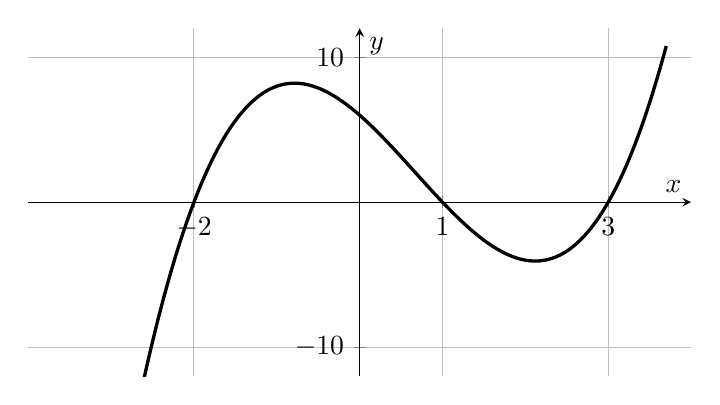
\begin{tikzpicture}
\begin{axis}[
    width=10cm,height=6cm,
    axis lines=middle,
    xmin=-4,xmax=4,
    ymin=-12,ymax=12,
    xlabel={$x$},ylabel={$y$},
    grid=both,
    samples=200,
    xtick={-2,1,3}
]
\addplot[very thick,domain=-3.2:3.7] {(x+2)*(x-1)*(x-3)};
\end{axis}
\end{tikzpicture}
\end{center}

\begin{question}
Geef de nulwaarden.

\begin{oplossing}
\[
x=-2,\quad x=1,\quad x=3.
\]
\end{oplossing}
\end{question}

\begin{question}
Voor welke \(x\) geldt \(f(x)>0\)?

\begin{oplossing}
\[
x\in]-2,1[\cup]3,+\infty[.
\]
\end{oplossing}
\end{question}

\begin{question}
Voor welke \(x\) geldt \(f(x)<0\)?

\begin{oplossing}
\[
x\in]-\infty,-2[\cup]1,3[.
\]
\end{oplossing}
\end{question}

\end{oefening}


\begin{oefening}[Van voorschrift naar tekentabel]{\oefB\ESS}

Stel telkens een tekentabel op.

\begin{question}
\[
f(x)=(x+3)(x-2).
\]

\begin{oplossing}
De nulwaarden zijn \(-3\) en \(2\).

\[
\begin{array}{c|ccccc}
x & ]-\infty,-3[ & -3 & ]-3,2[ & 2 & ]2,+\infty[\\
\hline
f(x)&+&0&-&0&+
\end{array}
\]
\end{oplossing}
\end{question}

\begin{question}
\[
g(x)=-(x-1)(x-4).
\]

\begin{oplossing}
De nulwaarden zijn \(1\) en \(4\).

\[
\begin{array}{c|ccccc}
x & ]-\infty,1[ & 1 & ]1,4[ & 4 & ]4,+\infty[\\
\hline
g(x)&-&0&+&0&-
\end{array}
\]
\end{oplossing}
\end{question}

\begin{question}
\[
h(x)=(x+1)^2(x-3).
\]

\begin{oplossing}
De nulwaarden zijn \(-1\) en \(3\).
Bij \(x=-1\) is er geen tekenwisseling.

\[
\begin{array}{c|ccccc}
x & ]-\infty,-1[ & -1 & ]-1,3[ & 3 & ]3,+\infty[\\
\hline
h(x)&-&0&-&0&+
\end{array}
\]
\end{oplossing}
\end{question}

\end{oefening}


\begin{oefening}[Domeinonderbreking of nulwaarde?]{\oefB\ESS}

Onderzoek het teken van

\[
f(x)=\frac{x-2}{x+1}.
\]

\begin{question}
Bepaal het domein en de nulwaarde.

\begin{oplossing}
\[
\operatorname{dom}f=\mathbb{R}\setminus\{-1\}.
\]

De nulwaarde volgt uit \(x-2=0\), dus \(x=2\).
\end{oplossing}
\end{question}

\begin{question}
Stel de tekentabel op.

\begin{oplossing}
\[
\begin{array}{c|ccccc}
x & ]-\infty,-1[ & -1 & ]-1,2[ & 2 & ]2,+\infty[\\
\hline
f(x)&+&\text{n.g.}&-&0&+
\end{array}
\]
\end{oplossing}
\end{question}

\begin{question}
Leg uit waarom \(x=-1\) geen nulwaarde is.

\begin{oplossing}
Voor \(x=-1\) is de noemer nul en bestaat \(f(-1)\) niet.
Een nulwaarde \(a\) moet voldoen aan \(f(a)=0\).
Daarom kan \(-1\) geen nulwaarde zijn.
\end{oplossing}
\end{question}

\end{oefening}


% ============================================================
% VERDIEPING
% ============================================================

\FVDsection{Verdieping — verbanden analyseren}

\begin{oefening}[Snijden of raken?]{\oefU\ESS}

Beschouw

\[
f(x)=(x+2)(x-1)^2(x-4).
\]

\begin{question}
Bepaal de nulwaarden.

\begin{oplossing}
\[
x=-2,\qquad x=1,\qquad x=4.
\]
\end{oplossing}
\end{question}

\begin{question}
Stel de tekentabel op.

\begin{oplossing}
Omdat \((x-1)^2\) aan beide zijden van \(1\) positief is,
verandert het teken daar niet.

\[
\begin{array}{c|ccccccc}
x & ]-\infty,-2[ & -2 & ]-2,1[ & 1 & ]1,4[ & 4 & ]4,+\infty[\\
\hline
f(x)&+&0&-&0&-&0&+
\end{array}
\]
\end{oplossing}
\end{question}

\begin{question}
Bij welke nulwaarde raakt de grafiek de \(x\)-as zonder van teken te veranderen?
Motiveer.

\begin{oplossing}
Bij \(x=1\).
De factor \((x-1)^2\) is aan beide zijden van \(1\) positief,
zodat het teken van het product daar niet verandert.
\end{oplossing}
\end{question}

\end{oefening}


\begin{oefening}[Van tekentabel naar grafische informatie]{\oefU\ESS}

Van een functie \(f\) is alleen de volgende tekentabel gegeven:

\[
\begin{array}{c|ccccccc}
x & ]-\infty,-3[ & -3 & ]-3,0[ & 0 & ]0,2[ & 2 & ]2,+\infty[\\
\hline
f(x)&-&0&+&0&+&0&-
\end{array}
\]

\begin{question}
Geef de nulwaarden.

\begin{oplossing}
\[
-3,\quad 0,\quad 2.
\]
\end{oplossing}
\end{question}

\begin{question}
Bij welke nulwaarde verandert het teken niet?

\begin{oplossing}
Bij \(x=0\): zowel links als rechts van \(0\) is \(f(x)>0\).
\end{oplossing}
\end{question}

\begin{question}
Beschrijf wat een mogelijke grafiek bij elk van de drie nulpunten doet.

\begin{oplossing}
Bij \(x=-3\) verandert het teken van negatief naar positief:
de grafiek gaat door de \(x\)-as.

Bij \(x=0\) blijft het teken positief:
de grafiek kan de \(x\)-as daar raken.

Bij \(x=2\) verandert het teken van positief naar negatief:
de grafiek gaat opnieuw door de \(x\)-as.
\end{oplossing}
\end{question}

\end{oefening}


\begin{oefening}[Vind de fout]{\oefU\ESS}

Een leerling onderzoekt

\[
f(x)=\frac{(x-3)(x+2)}{x-1}
\]

en schrijft:

\[
\text{``De bijzondere waarden zijn }-2,1,3,
\text{ dus alle drie zijn nulwaarden.''}
\]

Analyseer de redenering en stel de correcte tekentabel op.

\begin{oplossing}
De redenering is fout.

\[
x=-2\quad\text{en}\quad x=3
\]

maken de teller nul en zijn nulwaarden.

Voor \(x=1\) is de noemer nul. De functie is daar niet gedefinieerd,
dus \(1\) is geen nulwaarde.

\[
\begin{array}{c|ccccccc}
x & ]-\infty,-2[ & -2 & ]-2,1[ & 1 & ]1,3[ & 3 & ]3,+\infty[\\
\hline
f(x)&-&0&+&\text{n.g.}&-&0&+
\end{array}
\]
\end{oplossing}

\end{oefening}


\begin{oefening}[Grafiek, voorschrift en tekentabel vergelijken]{\oefU\ESS}

Drie leerlingen beschrijven dezelfde functie.

\begin{itemize}
    \item Leerling A: ``De nulwaarden zijn \(-2\) en \(3\). De functie
          is negatief tussen beide nulwaarden.''
    \item Leerling B: ``De tekentabel is \(+\;0\;-\;0\;+\).''
    \item Leerling C: ``De grafiek is een parabool die de \(x\)-as
          snijdt bij \(-2\) en \(3\) en buiten die nulwaarden boven
          de \(x\)-as ligt.''
\end{itemize}

\begin{question}
Leg uit waarom deze drie beschrijvingen met elkaar verenigbaar zijn.

\begin{oplossing}
Alle drie geven hetzelfde tekenverloop:

\[
f(x)>0 \text{ voor }x<-2\text{ en }x>3,
\]

\[
f(x)=0 \text{ voor }x=-2\text{ en }x=3,
\]

en

\[
f(x)<0 \text{ voor }-2<x<3.
\]

Ze gebruiken alleen verschillende voorstellingen:
woorden, een tekentabel en een grafische beschrijving.
\end{oplossing}
\end{question}

\begin{question}
Geef een eenvoudig functievoorschrift dat bij deze informatie past.

\begin{oplossing}
Bijvoorbeeld

\[
f(x)=(x+2)(x-3).
\]

Ook positieve veelvouden daarvan hebben hetzelfde tekenverloop.
\end{oplossing}
\end{question}

\end{oefening}


\begin{oefening}[Temperatuurverschil interpreteren]{\oefU\ESS}

Voor een experiment is

\[
D(t)=T_{\mathrm{proef}}(t)-T_{\mathrm{omgeving}}(t).
\]

Uit metingen volgt het tekenverloop

\[
\begin{array}{c|ccccc}
t & [0,4[ & 4 & ]4,11[ & 11 & ]11,15]\\
\hline
D(t)&-&0&+&0&-
\end{array}
\]

waarbij \(t\) in minuten wordt gemeten.

\begin{question}
Wat betekenen de nulwaarden \(4\) en \(11\) in de context?

\begin{oplossing}
Op \(t=4\) min en \(t=11\) min zijn de temperatuur van de
proefopstelling en de omgeving gelijk.
\end{oplossing}
\end{question}

\begin{question}
Wanneer is de proefopstelling warmer dan de omgeving?

\begin{oplossing}
Voor

\[
4<t<11.
\]
\end{oplossing}
\end{question}

\begin{question}
Formuleer de betekenis van \(D(t)<0\) zonder wiskundige symbolen.

\begin{oplossing}
De proefopstelling is dan kouder dan de omgeving.
Dat gebeurt gedurende de eerste vier minuten en opnieuw na minuut \(11\)
tot het einde van het beschouwde tijdsinterval.
\end{oplossing}
\end{question}

\end{oefening}


% ============================================================
% GEVORDERD
% ============================================================

\FVDsection{Gevorderd — combineren en modelleren}

\begin{oefening}[Ontwerp een functie]{\oefG}

Zoek een zo eenvoudig mogelijk veeltermvoorschrift \(f\) dat voldoet aan:

\begin{itemize}
    \item nulwaarden \(-2\), \(1\) en \(4\);
    \item bij \(x=1\) verandert het teken niet;
    \item voor \(x>4\) is \(f(x)>0\).
\end{itemize}

Stel de tekentabel op en leg uit waarom je voorschrift aan alle
voorwaarden voldoet.

\begin{oplossing}
Een mogelijke keuze is

\[
f(x)=(x+2)(x-1)^2(x-4).
\]

De factor \((x-1)^2\) zorgt ervoor dat \(1\) een nulwaarde is
zonder tekenwisseling.

\[
\begin{array}{c|ccccccc}
x & ]-\infty,-2[ & -2 & ]-2,1[ & 1 & ]1,4[ & 4 & ]4,+\infty[\\
\hline
f(x)&+&0&-&0&-&0&+
\end{array}
\]

Voor \(x>4\) zijn alle factoren positief, dus \(f(x)>0\).
\end{oplossing}

\end{oefening}


\begin{oefening}[Welke informatie is voldoende?]{\oefG}

Van een onbekende functie \(f\) weten we:

\[
f(-2)=0,\qquad f(3)=0.
\]

Een leerling besluit:

\[
f(x)<0\quad\text{voor }-2<x<3.
\]

Is die conclusie noodzakelijk juist?
Motiveer met twee verschillende voorbeelden van functies met
dezelfde nulwaarden.

\begin{oplossing}
Nee.

Bijvoorbeeld

\[
f(x)=(x+2)(x-3)
\]

is negatief tussen \(-2\) en \(3\).

Maar

\[
g(x)=-(x+2)(x-3)
\]

heeft dezelfde nulwaarden en is juist positief tussen \(-2\) en \(3\).

Nulwaarden alleen bepalen dus het volledige tekenverloop niet.
Er is bijkomende informatie nodig over het voorschrift of de grafiek.
\end{oplossing}

\end{oefening}


\begin{oefening}[Onderzoek met GeoGebra]{\oefG}

Voer in GeoGebra de familie

\[
f_a(x)=(x+2)(x-a)^2(x-4)
\]

in en maak \(a\) veranderlijk.

Onderzoek wat er gebeurt wanneer \(a\) van links naar rechts door
de andere nulwaarden beweegt.

Beschrijf:
\begin{enumerate}
    \item welke nulwaarden de functie heeft;
    \item bij welke nulwaarde geen tekenwisseling optreedt;
    \item hoe de tekentabel verandert wanneer \(a=-2\) of \(a=4\);
    \item welke informatie je uit de grafiek haalt en welke je
          algebraïsch controleert.
\end{enumerate}

\begin{oplossing}
Voor \(a\neq -2,4\) zijn de nulwaarden \(-2\), \(a\) en \(4\).
Door de kwadratische factor \((x-a)^2\) is er bij \(x=a\)
geen tekenwisseling.

Wanneer \(a=-2\) of \(a=4\), vallen factoren samen en verandert
de multipliciteit van die nulwaarde. Daardoor moet het tekenverloop
opnieuw worden onderzocht.

De grafiek helpt om het gedrag te voorspellen; de factorisatie maakt
algebraïsch zichtbaar waarom het teken wel of niet wisselt.
\end{oplossing}

\end{oefening}




\end{document}
